
%{{第三十九回}}{第三十九回}}

\chapter{村姥姥是信口开河\hspace{.5em}情哥哥偏寻根究底}

{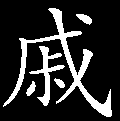
\includegraphics[width=3mm]{../Images/00005}  \kaishu 只为贫寒不拣行,富家趋入且逢迎。岂知着意无名利,便是三才最上乘。}

话说众人见平儿来了,都说:``你们奶奶作什么呢,怎么不来了?''平儿笑道:``他那里得空儿来。因为说没有好生吃得,又不得来,所以叫我来问还有没有,叫我要几个拿了家去吃罢。''湘云道:``有,多着呢。''忙令人拿了十个极大的。平儿道:``多拿几个团脐的。''众人又拉平儿坐,平儿不肯。李纨拉着他笑道:``偏要你坐。''拉着他身边坐下,端了一杯酒送到他嘴边。平儿忙喝了一口就要走。李纨道:``偏不许你去。显见得只有凤丫头,就不听我的话了。''说着又命嬷嬷们:``先送了盒子去,就说我留下平儿了。''那婆子一时拿了盒子回来说:``二奶奶说,叫奶奶和姑娘们别笑话要嘴吃。这个盒子里是方才舅太太那里送来的菱粉糕和鸡油卷儿,给奶奶姑娘们吃的。''又向平儿道:``说使你来你就贪住顽不去了。劝你少喝一杯儿罢。''平儿笑道:``多喝了又把我怎么样?''一面说,一面只管喝,又吃螃蟹。李纨揽着他笑道:``可惜这么个好体面模样儿,命却平常,只落得屋里使唤。不知道的人,谁不拿你当作奶奶太太看。''

平儿一面和宝钗湘云等吃喝,一面回头笑道:``奶奶,别只摸的我怪痒的。''李氏道:``嗳哟!这硬的是什么?''平儿道:``钥匙。''李氏道:``什么钥匙?要紧梯己东西怕人偷了去,却带在身上。我成日家和人说笑,有个唐僧取经,就有个白马来驮他;刘智远打天下,就有个瓜精来送盔甲;有个凤丫头,就有个你。你就是你奶奶的一把总钥匙,还要这钥匙作什么。''平儿笑道:``奶奶吃了酒,又拿了我来打趣着取笑儿了。''宝钗笑道:``这倒是真话。我们没事评论起人来,你们这几个都是百个里头挑不出一个来,妙在各人有各人的好处。''李纨道:``大小都有个天理。比如老太太屋里,要没那个鸳鸯如何使得。从太太起,那一个敢驳老太太的回,现在他敢驳回。偏老太太只听他一个人的话。老太太那些穿戴的,别人不记得,他都记得,要不是他经管着,不知叫人诓骗了多少去呢。那孩子心也公道,虽然这样,倒常替人说好话儿,还倒不依势欺人的。''惜春笑道:``老太太昨儿还说呢,他比我们还强呢。''平儿道:``那原是个好的,我们那里比的上他。''宝玉道:``太太屋里的彩霞,是个老实人。''探春道:``可不是,外头老实,心里有数儿。太太是那么佛爷似的,事情上不留心,他都知道。凡百一应事都是他提着太太行。连老爷在家出外去的一应大小事,他都知道。太太忘了,他背地里告诉太太。''李纨道:``那也罢了。''指着宝玉道:``这一个小爷屋里要不是袭人,你们度量到个什么田地!凤丫头就是楚霸王,也得这两只膀子好举千斤鼎。他不是这丫头,就得这么周到了!''平儿笑道:``先时陪了四个丫头,死的死,去的去,只剩下我一个孤鬼了。''李纨道:``你倒是有造化的。凤丫头也是有造化的。想当初你珠大爷在日,何曾也没两个人。你们看我还是那容不下人的?天天只见他两个不自在。所以你珠大爷一没了,趁年轻我都打发了。若有一个守得住,我倒有个膀臂。''说着滴下泪来。众人都道:``又何必伤心,不如散了倒好。''说着便都洗了手,大家约往贾母王夫人处问安。

众婆子丫头打扫亭子,收拾杯盘。袭人和平儿同往前去,让平儿到房里坐坐,再喝一杯茶。平儿说:``不喝茶了,再来吧。''说着便要出去。袭人又叫住问道:``这个月的月钱,连老太太和太太还没放呢,是为什么?''平儿见问,忙转身至袭人跟前,见方近无人,才悄悄说道:``你快别问,横竖再迟几天就放了。''袭人笑道:``这是为什么,唬得你这样?''平儿悄悄告诉他道:``这个月的月钱,我们奶奶早已支了,放给人使呢。等别处的利钱收了来,凑齐了才放呢。因为是你,我才告诉你,你可不许告诉一个人去。''袭人道:``难道他还短钱使,还没个足厌?何苦还操这心。''平儿笑道:``何曾不是呢。这几年拿着这一项银子,翻出有几百来了。他的公费月例又使不着,十两八两零碎攒了放出去,只他这梯己利钱,一年不到,上千的银子呢。''袭人笑道:``拿着我们的钱,你们主子奴才赚利钱,哄的我们呆呆的等着。''平儿道:``你又说没良心的话。你难道还少钱使?''袭人道:``我虽不少,只是我也没地方使去,就只预备我们那一个。''平儿道:``你倘若有要紧的事用钱使时,我那里还有几两银子,你先拿来使,明儿我扣下你的就是了。''袭人道:``此时也用不着,怕一时要用起来不够了,我打发人去取就是了。''

平儿答应着,一径出了园门,来至家内,只见凤姐儿不在房里。忽见上回来打抽丰的那刘姥姥和板儿又来了,坐在那边屋里,还有张材家的周瑞家的陪着,又有两三个丫头在地下倒口袋里的枣子倭瓜并些野菜。众人见他进来,都忙站起来了。{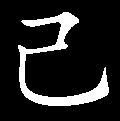
\includegraphics[width=3mm]{../Images/00003}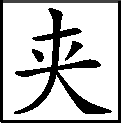
\includegraphics[width=3mm]{../Images/00012}\footnotesize \kaishu 妙文!上回是先见平儿后见凤姐,此则先见凤姐后见平儿也。何错综巧妙得情得理之至耶?}刘姥姥因上次来过,知道平儿的身分,忙跳下地来问``姑娘好'',又说:``家里都问好。早要来请姑奶奶的安看姑娘来的,因为庄家忙。好容易今年多打了两石粮食,瓜果菜蔬也丰盛。这是头一起摘下来的,并没敢卖呢,留的尖儿孝敬姑奶奶姑娘们尝尝。姑娘们天天山珍海味的也吃腻了,这个吃个野意儿,也算是我们的穷心。''

平儿忙道:``多谢费心。''又让坐,自己也坐了。又让``张婶子周大娘坐'',又令小丫头子倒茶去。周瑞张材两家的因笑道:``姑娘今儿脸上有些春色,眼圈儿都红了。''平儿笑道:``可不是。我原是不吃的,大奶奶和姑娘们只是拉着死灌,不得已喝了两盅,脸就红了。''张材家的笑道:``我倒想着要吃呢,又没人让我。明儿再有人请姑娘,可带了我去罢。''说着大家都笑了。

周瑞家的道:``早起我就看见那螃蟹了,一斤只好秤两个三个。这么三大篓,想是有七八十斤呢。''周瑞家的道:``若是上上下下只怕还不够。''平儿道:``那里够,不过都是有名儿的吃两个子。那些散众的,也有摸得着的,也有摸不着的。''刘姥姥道:``这样螃蟹,今年就值五分一斤。十斤五钱,五五二两五,三五一十五,再搭上酒菜,一共倒有二十多两银子。阿弥陀佛!这一顿的钱够我们庄家人过一年了。''

平儿因问:``想是见过奶奶了?''{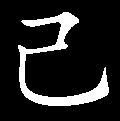
\includegraphics[width=3mm]{../Images/00003}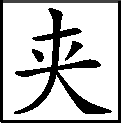
\includegraphics[width=3mm]{../Images/00012}\footnotesize \kaishu 写平儿伶俐如此。}刘姥姥道:``见过了,叫我们等着呢。''说着又往窗外看天气,{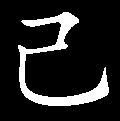
\includegraphics[width=3mm]{../Images/00003}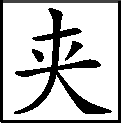
\includegraphics[width=3mm]{../Images/00012}\footnotesize \kaishu 是八月中,当开窗时,细致之甚。}说道:``天好早晚了,我们也去罢,别出不去城才是饥荒呢。''周瑞家的道:``这话倒是,我替你瞧瞧去。''说着一径去了,半日方来,笑道:``可是你老的福来了,竟投了这两个人的缘了。''平儿等问怎么样,周瑞家的笑道:``二奶奶在老太太的跟前呢。我原是悄悄的告诉二奶奶,`刘姥姥要家去呢,怕晚了赶不出城去。'二奶奶说:`大远的,难为他扛了那些沉东西来,晚了就住一夜明儿再去。'这可不是投上二奶奶的缘了。这也罢了,偏生老太太又听见了,问刘姥姥是谁。二奶奶便回明白了。老太太说:`我正想个积古的老人家说话儿,请了来我见一见。'这可不是想不到天上缘分了。''说着,催刘姥姥下来前去。刘姥姥道:``我这生像儿怎好见的。好嫂子,你就说我去了罢。''平儿忙道:``你快去罢,不相干的。我们老太太最是惜老怜贫的,比不得那个狂三诈四的那些人。想是你怯上,我和周大娘送你去。''说着,同周瑞家的引了刘姥姥往贾母这边来。

二门口该班的小厮们见了平儿出来,都站起来了,又有两个跑上来,赶着平儿叫``姑娘''。{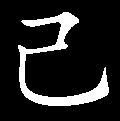
\includegraphics[width=3mm]{../Images/00003}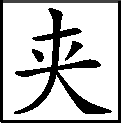
\includegraphics[width=3mm]{../Images/00012}\footnotesize \kaishu 想这一个``姑娘''非下称上之``姑娘''也,按北俗以姑母曰``姑姑'',南俗曰``娘娘'',此``姑娘''定是``姑姑''``娘娘''之称。每见大家风俗多有小童称少主妾曰``姑姑''``娘娘''者。按此书中若干人说话语气及动用器物饮食诸类,皆东西南北互相兼用,此``姑娘''之称,亦南北相兼而用无疑矣。}平儿问:``又说什么?''那小厮笑道:``这会子也好早晚了,我妈病了,等着我去请大夫。好姑娘,我讨半日假可使的?''平儿道:``你们倒好,都商议定了,一天一个告假,又不回奶奶,只和我胡缠。前儿住儿去了,二爷偏生叫他,叫不着,我应起来了,还说我作了情。你今儿又来了。''{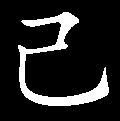
\includegraphics[width=3mm]{../Images/00003}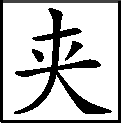
\includegraphics[width=3mm]{../Images/00012}\footnotesize \kaishu 分明几回没写到贾琏,今忽闲中一语,便补得贾琏这边天天闹热,令人却如看见听见一般。所谓不写之写也。刘姥姥眼中耳中又一番识面,奇妙之甚!}周瑞家的道:``当真的他妈病了,姑娘也替他应着,放了他罢。''平儿道:``明儿一早来。听着,我还要使你呢,再睡的日头晒着屁股再来!你这一去,带个信儿给旺儿,就说奶奶的话,问着他那剩的利钱。明儿若不交了来,奶奶也不要了,就越性送他使罢。''{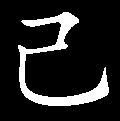
\includegraphics[width=3mm]{../Images/00003}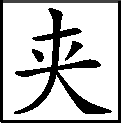
\includegraphics[width=3mm]{../Images/00012}\footnotesize \kaishu 交代过袭人的话,看他如此说,真比凤姐又甚一层。李纨之语不谬也。不知阿凤何等福得此一人。}那小厮欢天喜地答应去了。

平儿等来至贾母房中,彼时大观园中姊妹们都在贾母前承奉。{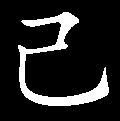
\includegraphics[width=3mm]{../Images/00003}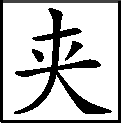
\includegraphics[width=3mm]{../Images/00012}\footnotesize \kaishu 妙极!连宝玉一并算入姊妹队中了。}刘姥姥进去,只见满屋里珠围翠绕,花枝招展,并不知都系何人。只见一张榻上歪着一位老婆婆,身后坐着一个纱罗裹的美人一般的一个丫鬟在那里捶腿,凤姐儿站着正说笑。{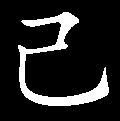
\includegraphics[width=3mm]{../Images/00003}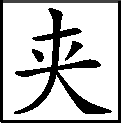
\includegraphics[width=3mm]{../Images/00012}\footnotesize \kaishu 奇奇怪怪文章。在刘姥姥眼中,以为阿凤至尊至贵,普天下人{(独)}{[}都{]}该站着说,阿凤独坐才是。如何今见阿凤独站哉?真妙文字。}刘姥姥便知是贾母了,忙上来陪着笑,福了几福,口里说:``请老寿星安。''{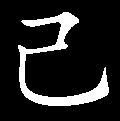
\includegraphics[width=3mm]{../Images/00003}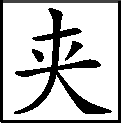
\includegraphics[width=3mm]{../Images/00012}\footnotesize \kaishu 更妙!贾母之号何其多耶?在诸人口中则曰``老太太'',在阿凤口中则曰``老祖宗'',在僧尼口中则曰``老菩萨'',在刘姥姥口中则曰``老寿星'',{(者)}{[}看{]}去似有数人,想去则皆贾母,难得如此各尽其妙。刘姥姥亦善应接。}贾母亦欠身问好,又命周瑞家的端过椅子来坐着。那板儿仍是怯人,不知问候。{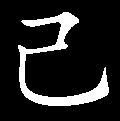
\includegraphics[width=3mm]{../Images/00003}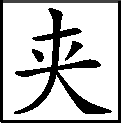
\includegraphics[width=3mm]{../Images/00012}\footnotesize \kaishu ``仍''字妙!盖有上文故也。不知教训者来看此句。}

贾母道:``老亲家,你今年多大年纪了?''{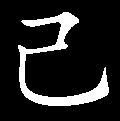
\includegraphics[width=3mm]{../Images/00003}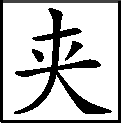
\includegraphics[width=3mm]{../Images/00012}\footnotesize \kaishu 神妙之极!看官至此必愁贾母以何相称,谁知公然曰``老亲家''。何等现成,何等大方,何等有情理。若云作者心中编出,余断断不信。何也?盖编得出者,断不能有这等情理。}刘姥姥忙立身答道:``我今年七十五了。''贾母向众人道:``这么大年纪了,还这么健朗。比我大好几岁呢。我要到这么大年纪,还不知怎么动不得呢。''刘姥姥笑道:``我们生来是受苦的人,老太太生来是享福的。若我们也这样,那些庄家活也没人作了。''贾母道:``眼睛牙齿都还好?''刘姥姥道:``都还好,就是今年左边的槽牙活动了。''贾母道:``我老了,都不中用了,眼也花,耳也聋,记性也没了。你们这些老亲戚,我都不记得了。亲戚们来了,我怕人笑我,我都不会,不过嚼的动的吃两口,睡一觉,闷了时和这些孙子孙女儿顽笑一回就完了。''刘姥姥笑道:``这正是老太太的福了。我们想这么着也不能。''贾母道:``什么福,不过是个老废物罢了。''说的大家都笑了。贾母又笑道:``我才听见凤哥儿说,你带了好些瓜菜来,叫他快收拾去了,我正想个地里现撷的瓜儿菜儿吃。外头买的,不像你们田地里的好吃。''刘姥姥笑道:``这是野意儿,不过吃个新鲜。依我们想鱼肉吃,只是吃不起。''贾母又道:``今儿既认着了亲,别空空儿的就去。不嫌我这里,就住一两天再去。我们也有个园子,园子里头也有果子,你明日也尝尝,带些家去,你也算看亲戚一趟。''

凤姐儿见贾母喜欢,也忙留道:``我们这里虽不比你们的场院大,空屋子还有两间。你住两天罢,把你们那里的新闻故事儿说些与我们老太太听听。''贾母笑道:``凤丫头别拿他取笑儿。他是乡屯里的人,老实,那里搁的住你打趣他。''说着,又命人去先抓果子与板儿吃。板儿见人多了,又不敢吃。贾母又命拿些钱给他,叫小幺儿们带他外头顽去。刘姥姥吃了茶,便把些乡村中所见所闻的事情说与贾母,贾母益发得了趣味。正说着,凤姐儿便令人来请刘姥姥吃晚饭。贾母又将自己的菜拣了几样,命人送过去与刘姥姥吃。

凤姐知道合了贾母的心,吃了饭便又打发过来。鸳鸯忙令老婆子带了刘姥姥去洗了澡,自己挑了两件随常的衣服令给刘姥姥换上。{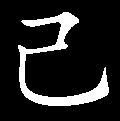
\includegraphics[width=3mm]{../Images/00003}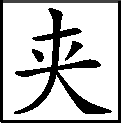
\includegraphics[width=3mm]{../Images/00012}\footnotesize \kaishu 一段鸳鸯身份、权势、心机,只写贾母也。}那刘姥姥那里见过这般行事,忙换了衣裳出来,坐在贾母榻前,又搜寻些话出来说。彼时宝玉姊妹们也都在这里坐着,他们何曾听见过这些话,自觉比那些瞽目先生说的书还好听。

那刘姥姥虽是个村野人,却生来的有些见识,况且年纪老了,世情上经历过的,见头一个贾母高兴,第二见这些哥儿姐儿们都爱听,便没了说的也编出些话来讲。因说道:``我们村庄上种地种菜,每年每日,春夏秋冬,风里雨里,那有个坐着的空儿,天天都是在那地头子上作歇马凉亭,什么奇奇怪怪的事不见呢。就像去年冬天,接连下了几天雪,地下压了三四尺深。我那日起的早,还没出房门,只听外头柴草响。我想着必定是有人偷柴草来了。我爬着窗户眼儿一瞧,却不是我们村庄上的人。''贾母道:``必定是过路的客人们冷了,见现成的柴,抽些烤火去也是有的。''刘姥姥笑道:``也并不是客人,所以说来奇怪。老寿星当个什么人?原来是一个十七八岁的极标致的一个小姑娘,梳着溜油光的头,穿着大红袄儿,白绫裙子------''{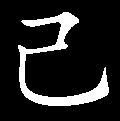
\includegraphics[width=3mm]{../Images/00003}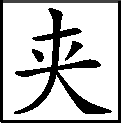
\includegraphics[width=3mm]{../Images/00012}\footnotesize \kaishu 刘姥姥的口气如此。}

刚说到这里,忽听外面人吵嚷起来,又说:``不相干的,别唬着老太太。''贾母等听了,忙问怎么了,丫鬟回说:``南院马棚里走了水,不相干,已经救下去了。''贾母最胆小的,听了这个话,忙起身扶了人出至廊上来瞧,只见东南上火光犹亮。贾母唬的口内念佛,忙命人去火神跟前烧香。王夫人等也忙都过来请安,又回说``已经下去了,老太太请进房去罢。''贾母足的看着火光息了方领众人进来。{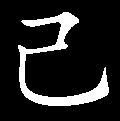
\includegraphics[width=3mm]{../Images/00003}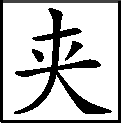
\includegraphics[width=3mm]{../Images/00012}\footnotesize \kaishu 一段为后回作引,然偏于宝玉爱听时截住。}宝玉且忙着问刘姥姥:``那女孩儿大雪地作什么抽柴草?倘或冻出病来呢?''贾母道:``都是才说抽柴草惹出火来了,你还问呢。别说这个了,再说别的罢。''宝玉听说,心内虽不乐,也只得罢了。

刘姥姥便又想了一篇,说道:``我们庄子东边庄上,有个老奶奶子,今年九十多岁了。他天天吃斋念佛,谁知就感动了观音菩萨夜里来托梦说:`你这样虔心,原来你该绝后的,如今奏了玉皇,给你个孙子。'原来这老奶奶只有一个儿子,这儿子也只一个儿子,好容易养到十七八岁上死了,哭的什么似的。后果然又养了一个,今年才十三四岁,生的雪团儿一般,聪明伶俐非常。可见这些神佛是有的。''这一席话,暗合了贾母王夫人的心事,连王夫人也都听住了。

宝玉心中只记挂着抽柴的故事,因闷闷的心中筹画。探春因问他:``昨日扰了史大妹妹,咱们回去商议着邀一社,又还了席,也请老太太赏菊花,何如?''宝玉笑道:``老太太说了,还要摆酒还史妹妹的席,叫咱们作陪呢。等着吃了老太太的,咱们再请不迟。''探春道:``越往前去越冷了,老太太未必高兴。''宝玉道:``老太太又喜欢下雨下雪的。不如咱们等下头场雪,请老太太赏雪岂不好?咱们雪下吟诗,也更有趣了。''林黛玉忙笑道:``咱们雪下吟诗?依我说,还不如弄一捆柴火,雪下抽柴,还更有趣儿呢。''说着,宝钗等都笑了。宝玉瞅了他一眼,也不答话。

一时散了,背地里宝玉足的拉了刘姥姥,细问那女孩儿是谁。刘姥姥只得编了告诉他道:``那原是我们庄北沿地埂子上有一个小祠堂里供的,不是神佛,当先有个什么老爷。''说着又想名姓。宝玉道:``不拘什么名姓,你不必想了,只说原故就是了。''刘姥姥道:``这老爷没有儿子,只有一位小姐,名叫茗玉。小姐知书识字,老爷太太爱如珍宝。可惜这茗玉小姐生到十七岁,一病死了。''宝玉听了,跌足叹惜,又问后来怎么样。刘姥姥道:``因为老爷太太思念不尽,便盖了这祠堂,塑了这茗玉小姐的像,派了人烧香拨火。如今日久年深的,人也没了,庙也烂了,那个像就成了精。''宝玉忙道:``不是成精,规矩这样人是虽死不死的。''刘姥姥道:``阿弥陀佛!原来如此。不是哥儿说,我们都当他成精。他时常变了人出来各村庄店道上闲逛。我才说这抽柴火的就是他了。我们村庄上的人还商议着要打了这塑像平了庙呢。''宝玉忙道:``快别如此。若平了庙,罪过不小。''刘姥姥道:``幸亏哥儿告诉我,我明儿回去告诉他们就是了。''宝玉道:``我们老太太、太太都是善人,合家大小也都好善喜舍,最爱修庙塑神的。我明儿做一个疏头,替你化些布施,你就做香头,攒了钱把这庙修盖,再装潢了泥像,每月给你香火钱烧香岂不好?''刘姥姥道:``若这样,我托那小姐的福,也有几个钱使了。''宝玉又问他地名庄名,来往远近,坐落何方。刘姥姥便顺口胡诌了出来。

宝玉信以为真,回至房中,盘算了一夜。次日一早,便出来给了茗烟几百钱,按着刘姥姥说的方向地名,着茗烟去先踏看明白,回来再做主意。那茗烟去后,宝玉左等也不来,右等也不来,急的热锅上的蚂蚁一般。好容易等到日落,方见茗烟兴兴头头的回来。宝玉忙道:``可有庙了?''茗烟笑道:``爷听的不明白,叫我好找。那地名座落不似爷说的一样,所以找了一日,找到东北上田埂子上才有一个破庙。''宝玉听说,喜的眉开眼笑,忙说道:``刘姥姥有年纪的人,一时错记了也是有的。你且说你见的。''茗烟道:``那庙门却倒是朝南开,也是稀破的。我找的正没好气,一见这个,我说`可好了',连忙进去。一看泥胎,唬的我跑出来了,活似真的一般。''宝玉喜的笑道:``他能变化人了,自然有些生气。''茗烟拍手道:``那里有什么女孩儿,竟是一位青脸红发的瘟神爷。''宝玉听了,啐了一口,骂道:``真是一个无用的杀才!这点子事也干不来。''茗烟道:``二爷又不知看了什么书,或者听了谁的混话,信真了,把这件没头脑的事派我去碰头,怎么说我没用呢?''宝玉见他急了,忙抚慰他道:``你别急。改日闲了你再找去。若是他哄我们呢,自然没了,若真是有的,你岂不也积了阴骘。我必重重的赏你。''正说着,只见二门上的小厮来说:``老太太房里的姑娘们站在二门口找二爷呢。''

{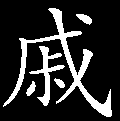
\includegraphics[width=3mm]{../Images/00005}  \kaishu 总评:此回第一写势利之好财,第二写穷苦趋势之求财。且文章不得雷同,先既有诗社,而今不得不用套坡公听鬼之遗事,以振其馀响,即此以点染宝玉之痴。其文真如环转,无端倪可指。}
